\chapter{Introduzione}
%\addcontentsline{toc}{chapter}{Introduzione al corso}

Gli obiettivi di questo capitolo sono: 
\begin{itemize}
    \item capire cos'è l'ingegneria del software e perché è importante; 
    \item comprendere che lo sviluppo di diversi tipi di sistemi software può richiedere diverse tecniche di ingegneria del software; 
    \item comprendere alcune questioni etiche e professionali importanti per gli ingegneri del software; \item introduzione di tre sistemi, di diversa tipologia, che verranno utilizzati come esempi in tutto il corso.
\end{itemize}

\begin{redbar}
L'\textbf{ingegneria del software} è un campo che si occupa dello sviluppo professionale di software utilizzando teorie, metodi e strumenti specifici.
\end{redbar}

È una disciplina che ha acquisito sempre maggiore importanza in tutte le economie avanzate. Con l'espansione tecnologica e l'automazione di molti sistemi, sempre più operazioni dipendono da software avanzati. Questa dipendenza ha reso l'ingegneria del software un fattore determinante per lo sviluppo economico, influenzando una parte significativa del Prodotto Interno Lordo (PIL) dei paesi sviluppati.

Uno degli aspetti centrali dell'ingegneria del software riguarda la gestione dei costi. Quando si sviluppa un sistema informatico, le spese legate al software spesso superano di gran lunga quelle del hardware. Questo fenomeno è particolarmente evidente nei personal computer, dove il costo di licenze e aggiornamenti del software può superare quello delle componenti fisiche della macchina. Tuttavia, uno degli aspetti più onerosi è rappresentato dai costi di manutenzione del software, che superano quelli di sviluppo iniziale.

Poiché le nuove tecniche di ingegneria del software ci aiutano a costruire sistemi più grandi e complessi, le richieste devono essere costruite e fornite più rapidamente; sono richiesti sistemi più grandi e ancora più complessi. È abbastanza facile scrivere programmi per computer senza utilizzare metodi e tecniche di ingegneria del software. Molte aziende, infatti, si sono spostate verso lo sviluppo di software man mano che i loro prodotti e servizi si sono evoluti. Non utilizzando metodi di ingegneria del software nel loro lavoro quotidiano il loro software è spesso più costoso e meno affidabile di quanto dovrebbe essere.

\section{Sviluppo software professionale}
La stragrande maggioranza dello sviluppo software è un'attività professionale in cui il software viene sviluppato per scopi aziendali specifici, per essere incluso in altri dispositivi o come prodotti software come sistemi informativi. Il software professionale, destinato a essere utilizzato da qualcuno oltre al suo sviluppatore, è solitamente sviluppato da team piuttosto che da singoli individui e viene mantenuto e modificato nel corso della sua vita.

\begin{table}[ht]
\centering
\rowcolors{2}{lightblue}{lightgray}
\begin{tabular}{|p{6cm}|p{9cm}|}
\hline
\rowcolor{headerblue}
\textbf{\textcolor{white}{Domanda}} & \textbf{\textcolor{white}{Risposta}} \\
\hline
Cos'è il software? & Programmi per computer e documentazione associata. I prodotti software possono essere sviluppati per un cliente specifico o per il mercato generale. \\
\hline
Quali sono le caratteristiche di un buon software? & Un buon software deve fornire le funzionalità richieste e le prestazioni attese dall'utente, e deve essere mantenibile, affidabile e facile da usare. \\
\hline
Cos'è l'ingegneria del software? & L'ingegneria del software è una disciplina ingegneristica che si occupa di tutti gli aspetti della produzione di software. \\
\hline
Quali sono le attività fondamentali dell'ingegneria del software? & Specifica del software, sviluppo del software, validazione del software ed evoluzione del software. \\
\hline
Qual è la differenza tra ingegneria del software e informatica? & L'informatica si concentra sulla teoria e sui fondamenti; l'ingegneria del software si occupa delle questioni pratiche dello sviluppo e della distribuzione di software utile. \\
\hline
Qual è la differenza tra ingegneria del software e ingegneria dei sistemi? & L'ingegneria dei sistemi si occupa di tutti gli aspetti dello sviluppo di sistemi basati su computer, compresi hardware, software e ingegneria dei processi. L'ingegneria del software è parte di questo processo più generale. \\
\hline
Quali sono le principali sfide dell'ingegneria del software? & Affrontare una crescente diversità, richieste di tempi di consegna ridotti e lo sviluppo di software affidabile. \\
\hline
Quali sono i costi dell'ingegneria del software? & Circa il 60\% dei costi del software sono costi di sviluppo; il 40\% sono costi di test. Per il software su misura, i costi di evoluzione spesso superano i costi di sviluppo. \\
\hline
Quali sono le migliori tecniche e metodi di ingegneria del software? & Anche se tutti i progetti software devono essere gestiti e sviluppati professionalmente, diverse tecniche sono appropriate per diversi tipi di sistema. Ad esempio, i giochi dovrebbero sempre essere sviluppati tramite una serie di prototipi, mentre i sistemi di controllo critici per la sicurezza richiedono una specifica completa e analizzabile. Non si può quindi affermare che un metodo sia migliore di un altro. \\
\hline
Quali differenze ha introdotto il Web nell'ingegneria del software? & Il Web ha portato alla disponibilità di servizi software e alla possibilità di sviluppare sistemi distribuiti basati su servizi. Lo sviluppo di sistemi Web ha portato importanti progressi nei linguaggi di programmazione e nel riutilizzo del software. \\
\hline
\end{tabular}
\caption{Domande frequenti sul software}
\end{table}

Molte persone pensano che il software sia semplicemente un altro termine per indicare i programmi per computer. Tuttavia, quando parliamo di ingegneria del software, il software non è solo i programmi stessi, ma anche tutta la documentazione associata e i dati di configurazione necessari per far funzionare correttamente questi programmi.


Gli ingegneri del software si occupano dello sviluppo di prodotti software (cioè, software che possono essere venduti a un cliente). Esistono due tipi di prodotti software:
\begin{enumerate}
    \item \textit{Prodotti generici:} Questi sono sistemi autonomi prodotti da un'organizzazione di sviluppo e venduti sul mercato aperto a qualsiasi cliente che sia in grado di acquistarli. Esempi di questo tipo di prodotto includono software per PC come database, elaboratori di testi, pacchetti di disegno e strumenti di gestione di progetti. Include anche le cosiddette applicazioni verticali progettate per scopi specifici come i sistemi informativi per biblioteche, i sistemi contabili o i sistemi per la gestione delle cartelle cliniche dentali.
    \item \textit{Prodotti personalizzati:} Questi sono sistemi commissionati da un particolare cliente. Un'azienda di sviluppo software sviluppa il software appositamente per quel cliente. Esempi di questo tipo di software includono sistemi di controllo per dispositivi elettronici, sistemi scritti per supportare un particolare processo aziendale e sistemi di controllo del traffico aereo.
\end{enumerate}
Una differenza importante tra questi tipi di software è che, nei prodotti generici, l'organizzazione che sviluppa il software controlla la specifica del software. Per i prodotti personalizzati, la specifica viene solitamente sviluppata e controllata dall'organizzazione che acquista il software. I sviluppatori devono lavorare su quella specifica.

\begin{table}[ht]
\centering
\rowcolors{2}{lightblue}{lightgray}
\begin{tabular}{|p{6cm}|p{9cm}|}
\hline
\rowcolor{headerblue}
\textbf{\textcolor{white}{Caratteristiche del prodotto}} & \textbf{\textcolor{white}{Descrizione}} \\
\hline
Manutenibilità & Il software dovrebbe essere scritto in modo tale da poter evolvere per soddisfare le esigenze in continuo cambiamento dei clienti. Questo è un attributo critico perché il cambiamento del software è un requisito inevitabile in un ambiente aziendale in evoluzione.
\\
\hline
Affidabilità e sicurezza & L'affidabilità del software include una serie di caratteristiche come affidabilità, sicurezza e sicurezza operativa. Il software affidabile non dovrebbe causare danni fisici o economici in caso di guasto del sistema. Gli utenti malintenzionati non dovrebbero essere in grado di accedere o danneggiare il sistema.
\\
\hline
Efficienza & Il software non dovrebbe fare un uso inutile delle risorse di sistema, come la memoria e i cicli del processore. L'efficienza include quindi la reattività, il tempo di elaborazione, l'utilizzo della memoria, ecc.
\\
\hline
Accettabilità & Il software deve essere accettabile per il tipo di utenti a cui è destinato. Ciò significa che deve essere comprensibile, utilizzabile e compatibile con altri sistemi che utilizzano.
\\
\hline
\end{tabular}
\caption{Attributi essenziali di un buon software}
\end{table}

\subsection{Ingegneria del software}
L'ingegneria del software è una disciplina ingegneristica che si occupa di tutti gli aspetti della produzione di software, dalle prime fasi della specifica del sistema fino alla manutenzione del sistema dopo che è stato messo in uso. In questa definizione, ci sono due frasi chiave:
\begin{enumerate}
    \item \textit{Disciplina ingegneristica:} Gli ingegneri applicano teorie, metodi e strumenti quando appropriato, ma li usano in modo selettivo e cercano sempre soluzioni ai problemi, anche quando non esistono teorie e metodi applicabili. Inoltre, gli ingegneri riconoscono che devono lavorare con vincoli organizzativi e finanziari, quindi cercano soluzioni all'interno di questi limiti.
    \item \textit{Tutti gli aspetti della produzione del software:} L'ingegneria del software non si occupa solo dei processi tecnici di sviluppo software, ma include anche attività come la gestione dei progetti software e lo sviluppo di strumenti, metodi e teorie per supportare la produzione di software.
\end{enumerate}

L'ingegneria del software è importante per due motivi:
\begin{enumerate}
    \item Sempre di più, individui e società si affidano a sistemi software avanzati. Dobbiamo essere in grado di produrre sistemi affidabili e sicuri in modo economico e rapido.
    \item A lungo termine, è di solito più economico utilizzare metodi e tecniche di ingegneria del software per i sistemi software piuttosto che scrivere semplicemente i programmi come fossero progetti di programmazione personali. Per la maggior parte dei tipi di sistemi, i costi maggiori sono quelli legati alle modifiche del software una volta che è stato messo in uso.
\end{enumerate}
L'approccio sistematico utilizzato nell'ingegneria del software è talvolta chiamato processo software. Un processo software è una sequenza di attività che porta alla produzione di un prodotto software. Ci sono quattro attività fondamentali comuni a tutti i processi software:
\begin{enumerate}
    \item \textit{Specificazione del software}, in cui i clienti e gli ingegneri definiscono il software da produrre e i vincoli sul suo funzionamento.
    \item \textit{Sviluppo del software}, in cui il software viene progettato e programmato.
    \item \textit{Validazione del software}, in cui il software viene verificato per garantire che corrisponda ai requisiti del cliente.
    \item \textit{Evoluzione del software}, in cui il software viene modificato per riflettere le esigenze dei clienti e del mercato in evoluzione.
\end{enumerate}

Ci sono quattro questioni generali che influenzano molti tipi di software:
\begin{enumerate}
    \item \textit{Eterogeneità:} Sempre più spesso i sistemi devono operare come sistemi distribuiti su reti che includono diversi tipi di computer e dispositivi mobili. Il software deve integrarsi con sistemi legacy scritti in diversi linguaggi di programmazione.
    \item \textit{Cambiamento aziendale e sociale:} Il mondo aziendale e sociale sta cambiando rapidamente. È necessario essere in grado di modificare il software esistente e sviluppare rapidamente nuovo software.
    \item \textit{Sicurezza e fiducia:} Poiché il software è strettamente connesso a tutti gli aspetti della nostra vita, è essenziale che ci si possa fidare di esso.
    \item \textit{Scala:} Il software deve essere sviluppato su una vasta gamma di scale, da sistemi embedded molto piccoli in dispositivi portatili o indossabili fino a sistemi basati su cloud e su scala Internet che servono una comunità globale.
\end{enumerate}

\subsection{Diversità nell'ingegneria del software}
Non esiste un metodo universale di ingegneria del software adatto a tutti i sistemi e le aziende. Piuttosto, nel corso degli ultimi 50 anni si è evoluta una vasta gamma di metodi e strumenti di ingegneria del software, ognuno adatto a differenti contesti.

Uno dei fattori principali che influenzano la scelta dei metodi di ingegneria del software è il tipo di applicazione che si sta sviluppando. Di seguito sono riportati i principali tipi di applicazioni:
\begin{enumerate}
    \item \textit{Applicazioni stand-alone:} Sistemi che funzionano su un computer locale senza bisogno di una connessione di rete.
    \item \textit{Applicazioni interattive basate su transazioni:} Applicazioni che vengono eseguite su un computer remoto e a cui gli utenti accedono da PC o terminali. Come applicazioni web di e-commerce, sistemi aziendali o servizi cloud.
    \item \textit{Sistemi di controllo embedded:} Sistemi software che gestiscono dispositivi hardware. Numericamente, probabilmente ci sono più sistemi embedded di qualsiasi altro tipo di sistema.
    \item \textit{Sistemi batch:} Sistemi aziendali progettati per elaborare dati in grandi blocchi. Elaborano un gran numero di input individuali per creare output corrispondenti.
    \item \textit{Sistemi di intrattenimento:} Sistemi progettati per uso personale e destinati a intrattenere l'utente.
    \item \textit{Sistemi di modellazione e simulazione:} Sistemi utilizzati per modellare processi fisici o situazioni.
    \item \textit{Sistemi di raccolta dati:} Sistemi che raccolgono dati dall'ambiente attraverso sensori e inviano tali dati ad altri sistemi per l'elaborazione.
    \item \textit{Sistemi di sistemi:} Sistemi composti da altri sistemi software.
\end{enumerate}
Nonostante questa diversità, esistono alcuni principi fondamentali dell'ingegneria del software che si applicano a tutti i tipi di sistemi:
\begin{enumerate}
    \item \textit{Processo di sviluppo gestito:} Il processo di sviluppo deve essere pianificato, e l'organizzazione deve avere un'idea chiara di cosa sarà prodotto e quando.
    \item \textit{Affidabilità e prestazioni:} Il software deve comportarsi come previsto senza guasti, essere sicuro e performante.
    \item \textit{Gestione delle specifiche:} È essenziale capire e gestire le aspettative dei clienti per fornire un sistema utile entro i limiti di tempo e budget.
    \item \textit{Riutilizzo delle risorse esistenti:} Dove possibile, è preferibile riutilizzare software esistente piuttosto che scrivere nuovo codice.
\end{enumerate}

\subsection{Ingegneria del software e Web}
L'evoluzione del World Wide Web ha avuto un impatto significativo sullo sviluppo del software. Inizialmente, il Web fungeva principalmente come archivio di informazioni accessibile a tutti e non influenzava direttamente i sistemi software, che operavano localmente all'interno delle organizzazioni. Tuttavia, intorno all'anno 2000, il Web ha iniziato a cambiare con l'aggiunta di maggiore funzionalità ai browser, permettendo la creazione di sistemi web-based accessibili tramite un browser web anziché un'interfaccia utente specifica. Questo ha favorito la nascita di nuovi prodotti software e servizi innovativi, spesso finanziati dalla pubblicità, senza che gli utenti pagassero direttamente per l'accesso.

La capacità dei browser di eseguire piccoli programmi e gestire alcune elaborazioni locali ha portato all'evoluzione del software aziendale. Invece di distribuire e installare il software sui PC degli utenti, esso veniva implementato su server web, riducendo notevolmente i costi di aggiornamento e distribuzione. Questo cambiamento ha spinto molte aziende a passare all'interazione web-based con i propri sistemi.

Negli ultimi anni si è diffusa l'idea secondo cui il software non viene eseguito localmente sui computer ma su cloud computing accessibili via Internet. I cloud computing sono grandi insiemi di sistemi informatici collegati, condivisi da molti utenti, che pagano in base all'uso del software.

Questi cambiamenti hanno modificato anche il modo in cui i sistemi web-based vengono progettati:
\begin{enumerate}
    \item Il riutilizzo di componenti preesistenti è diventato il metodo dominante per costruire sistemi web-based. Quando si costruiscono questi sistemi, si pensa a come assemblarli da componenti software e sistemi preesistenti.
    \item È ormai riconosciuto che non è pratico definire in anticipo tutte le specifiche per questi sistemi. Pertanto, devono essere sviluppati e rilasciati in modo incrementale.
    \item Il software può essere implementato utilizzando l'ingegneria del software orientata ai servizi, in cui i componenti software sono servizi Web autonomi.
    \item Sono emerse tecnologie di sviluppo di interfacce come AJAX e HTML5 che supportano la creazione di interfacce avanzate all'interno di un browser web.
\end{enumerate}
Nonostante queste differenze, i concetti fondamentali dell'ingegneria del software rimangono applicabili anche ai sistemi web-based.

\section{Etica dell'ingegneria del software}
L'ingegneria del software comporta responsabilità più ampie della semplice applicazione di competenze tecniche. Gli ingegneri del software devono comportarsi in modo onesto ed eticamente responsabile se vogliono essere rispettati come professionisti. Il comportamento etico è più che semplicemente rispettare la legge, ma implica seguire una serie di principi che sono moralmente corretti. Tuttavia, ci sono aree in cui gli standard di comportamento accettabili non sono vincolati dalla legge, ma dalla più tenue nozione di responsabilità professionale. Alcuni di questi includono:
\begin{enumerate}
    \item \textit{Riservatezza:} Dovresti normalmente rispettare la riservatezza dei tuoi datori di lavoro o clienti, indipendentemente dal fatto che sia stato firmato un accordo di riservatezza formale o meno.
    \item \textit{Competenza:} Non dovresti rappresentare falsamente il tuo livello di competenza. Non dovresti accettare consapevolmente lavori che siano al di fuori delle tue competenze.
    \item \textit{Diritti di proprietà intellettuale:} Dovresti essere a conoscenza delle leggi locali che governano l'uso della proprietà intellettuale, come brevetti e diritti d'autore. Dovresti prestare attenzione a garantire che la proprietà intellettuale dei datori di lavoro e dei clienti sia protetta.
    \item \textit{Uso improprio dei computer:} Non dovresti utilizzare le tue competenze tecniche per abusare dei computer altrui. L'uso improprio dei computer varia da comportamenti relativamente banali (giocare su una macchina del datore di lavoro) a questioni estremamente serie (diffusione di virus o altri malware).
\end{enumerate}
Le società e le istituzioni professionali hanno un ruolo importante nel definire gli standard etici. Organizzazioni come l'ACM (Association for Computing Machinery), l'IEEE (Institute of Electrical and Electronic Engineers) e la British Computer Society pubblicano un codice di condotta professionale o un codice etico. I membri di queste organizzazioni si impegnano a seguire tale codice quando si iscrivono. Questi codici di condotta riguardano generalmente comportamenti etici fondamentali. Il Codice contiene otto Principi relativi al comportamento e alle decisioni prese dai professionisti dell'ingegneria del software, inclusi praticanti, educatori, manager, supervisori e responsabili politici, oltre a tirocinanti e studenti della professione.

\begin{center}
\begin{minipage}{0.9\textwidth}
\textit{I computer hanno un ruolo centrale e in crescita nel commercio, nell'industria, nel governo, nella medicina, nell'istruzione, nell'intrattenimento e nella società in generale. Gli ingegneri del software sono coloro che contribuiscono, attraverso la partecipazione diretta o l'insegnamento, all'analisi, alla specifica, alla progettazione, allo sviluppo, alla certificazione, alla manutenzione e al collaudo dei sistemi software. A causa dei loro ruoli nello sviluppo dei sistemi software, gli ingegneri del software hanno significative opportunità di fare del bene o causare danno, di abilitare gli altri a fare del bene o causare danno, o di influenzare gli altri a fare del bene o causare danno. Per garantire, per quanto possibile, che i loro sforzi vengano utilizzati per il bene, gli ingegneri del software devono impegnarsi a fare dell'ingegneria del software una professione benefica e rispettata. In conformità a tale impegno, gli ingegneri del software devono aderire al seguente Codice di Etica e Pratica Professionale.}
\end{minipage}
\end{center}

\begin{center}
\begin{minipage}{\textwidth} % Larghezza della minipage (50% della larghezza del testo)
\colorbox{lightgray}{ % Crea uno sfondo grigio chiaro
\parbox{\linewidth}{ % Parbox per assicurarsi che il testo si adatti
\textbf{Codice Etico e Pratica Professionale dell'Ingegneria del Software}\\
Gruppo di Lavoro Congiunto ACM/IEEE-CS sull'Etica e le Pratiche Professionali nell'Ingegneria del Software\\
\textbf{PREAMBOLO}\\
La versione breve del codice riassume le aspirazioni a un alto livello di astrazione; le clausole incluse nella versione completa forniscono esempi e dettagli su come queste aspirazioni cambiano il nostro modo di agire come professionisti dell'ingegneria del software. Senza le aspirazioni, i dettagli possono diventare legalistici e tediosi; senza i dettagli, le aspirazioni possono risultare altisonanti ma vuote; insieme, aspirazioni e dettagli formano un codice coerente.

Gli ingegneri del software si impegneranno a fare dell'analisi, della specifica, della progettazione, dello sviluppo, del collaudo e della manutenzione del software una professione benefica e rispettata. In conformità con il loro impegno per la salute, la sicurezza e il benessere del pubblico, gli ingegneri del software devono aderire ai seguenti Otto Principi:
\begin{enumerate}
    \item PUBBLICO — Gli ingegneri del software agiranno in modo coerente con l'interesse pubblico.
    \item CLIENTE E DATORE DI LAVORO — Gli ingegneri del software agiranno in un modo che sia nel miglior interesse del loro cliente e datore di lavoro, in coerenza con l'interesse pubblico.
    \item PRODOTTO — Gli ingegneri del software garantiranno che i loro prodotti e le modifiche correlate soddisfino i più elevati standard professionali possibili.
    \item GIUDIZIO — Gli ingegneri del software manterranno integrità e indipendenza nel loro giudizio professionale.
    \item GESTIONE — I manager e i leader nell'ingegneria del software si iscriveranno e promuoveranno un approccio etico alla gestione dello sviluppo e della manutenzione del software.
    \item PROFESSIONE — Gli ingegneri del software promuoveranno l'integrità e la reputazione della professione in coerenza con l'interesse pubblico.
    \item COLLEGHI — Gli ingegneri del software saranno giusti e solidali nei confronti dei loro colleghi.
    \item SE STESSI — Gli ingegneri del software parteciperanno a un apprendimento continuo riguardante la pratica della loro professione e promuoveranno un approccio etico alla pratica della professione.
\end{enumerate}
}}
\end{minipage}
\end{center}

\section{Casi di studio}
Per illustrare i concetti dell'ingegneria del software, utilizzo esempi tratti da quattro diverse tipologie di sistema.
\begin{enumerate}
    \item \textit{Una pompa per insulina personale:} Un sistema incorporato in una pompa per insulina utilizzata dai diabetici per mantenere il controllo della glicemia.
    \item \textit{Un sistema di gestione dei casi di salute mentale:} Mentcare. Un sistema utilizzato per conservare i registri delle persone che ricevono cure per problemi di salute mentale.
    \item \textit{Una stazione meteorologica per aree selvagge:} Un sistema di raccolta dati che raccoglie dati sulle condizioni meteorologiche in aree remote.
    \item \textit{iLearn:} un ambiente di apprendimento digitale. Un sistema per supportare l'apprendimento nelle scuole.
\end{enumerate}

\subsection*{Sistema di controllo della pompa di insulina}
Una pompa di insulina è un sistema medico che simula il funzionamento del pancreas. Il software che controlla questo sistema è un sistema embedded che raccoglie informazioni da un sensore di glicemia e calcola la quantità di insulina necessaria da iniettare. Il calcolo basato sulla velocità di variazione dei livelli di glicemia. Quindi una pompa somministra una dose controllata di insulina a un utente.

Un controllo irregolare può portare a livelli molto bassi di glucosio nel sangue (se c'è troppa insulina) o a livelli molto alti di zucchero nel sangue (se c'è troppo poca insulina). Un basso livello di glucosio nel sangue è, a breve termine, una condizione più grave poiché può comportare malfunzionamenti temporanei del cervello e, infine, incoscienza e morte. A lungo termine, tuttavia, livelli costantemente elevati di glucosio nel sangue possono portare a danni agli occhi, danni ai reni e problemi cardiaci.

La figura \ref{fig:insulin-pump-hardware} mostra i componenti hardware e l'organizzazione della pompa di insulina. Il sensore del sangue misura la conduttività elettrica del sangue in diverse condizioni, questi valori possono essere correlati al livello di zucchero nel sangue. La pompa di insulina fornisce un'unità di insulina in risposta a un singolo impulso proveniente da un controller. Pertanto, per somministrare 10 unità di insulina, il controller invia 10 impulsi alla pompa. La figura \ref{fig:activity-model-insulin-pump} è un modello di attività UML (Unified Modeling Language) che illustra come il software trasforma un livello di zucchero nel sangue in una sequenza di comandi che azionano la pompa di insulina.

\begin{figure}[ht]
    \centering
    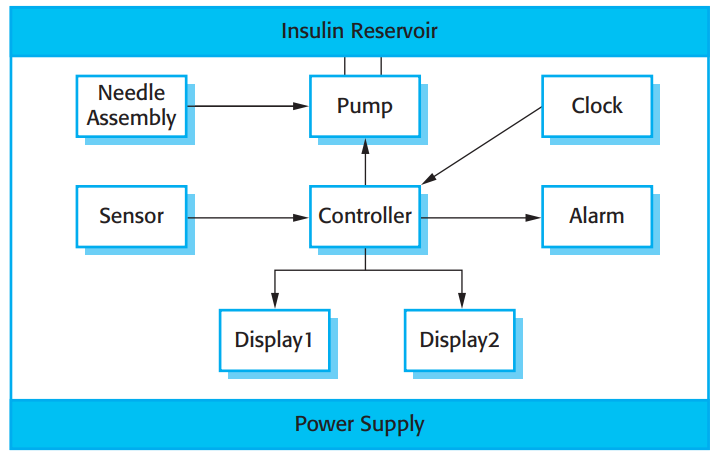
\includegraphics[width=0.6\linewidth]{images/insulin-pump-hardware.PNG}
    \caption{Hardware per pompe di insulina}
    \label{fig:insulin-pump-hardware}
\end{figure}

\begin{figure}[ht]
    \centering
    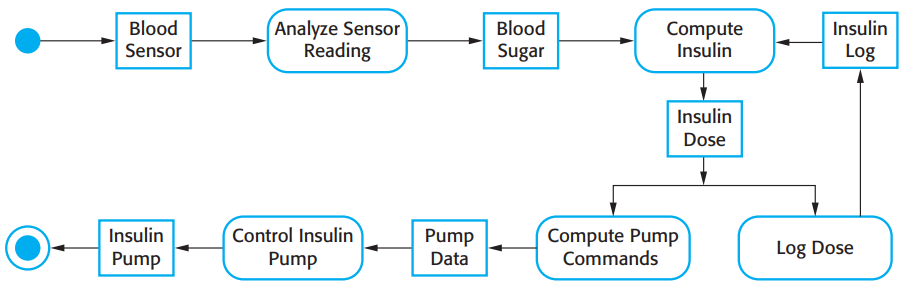
\includegraphics[width=0.7\linewidth]{images/activity-model-insulin-pump.PNG}
    \caption{Modello di attività della pompa per insulina}
    \label{fig:activity-model-insulin-pump}
\end{figure}

Chiaramente, questo è un sistema critico per la sicurezza. Questo sistema deve quindi soddisfare due requisiti essenziali di alto livello:
\begin{enumerate}
    \item Il sistema deve essere disponibile per somministrare insulina quando necessario.
    \item Il sistema deve funzionare in modo affidabile e fornire la giusta quantità di insulina per controbilanciare il livello attuale di zucchero nel sangue.
\end{enumerate}
Il sistema deve quindi essere progettato e implementato per garantire che soddisfi sempre questi requisiti.

\subsection*{Sistema informativo per i pazienti per l'assistenza sanitaria mentale}
Un sistema informativo per pazienti a supporto della cura della salute mentale (il sistema Mentcare) è un sistema informativo medico che gestisce informazioni sui pazienti affetti da problemi di salute mentale e sui trattamenti che hanno ricevuto. La maggior parte dei pazienti con problemi di salute mentale non richiede un trattamento ospedaliero dedicato, ma deve recarsi regolarmente presso cliniche specialistiche dove possono incontrare un medico che ha una conoscenza approfondita dei loro problemi. Per facilitare l'accesso dei pazienti, queste cliniche non sono gestite solo negli ospedali. Possono anche essere tenute presso ambulatori medici locali o centri comunitari.

Il sistema Mentcare (Figura \ref{fig:organization-mhc-pms}) è un sistema informativo per pazienti destinato all'uso nelle cliniche. Utilizza un database centralizzato di informazioni sui pazienti, ma è stato anche progettato per funzionare su un laptop, in modo da poter essere accessibile e utilizzato in luoghi che non hanno connettività di rete sicura. Quando i sistemi locali hanno accesso alla rete sicura, utilizzano le informazioni sui pazienti presenti nel database, ma possono scaricare e utilizzare copie locali delle cartelle cliniche quando sono disconnessi.

\begin{figure}[ht]
    \centering
    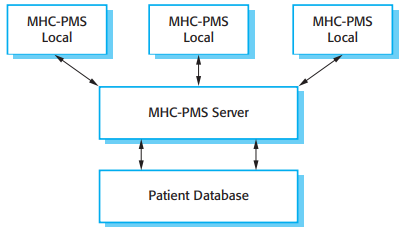
\includegraphics[width=0.5\linewidth]{images/organization-mhc-pms.PNG}
    \caption{L'organizzazione del MHC-PMS}
    \label{fig:organization-mhc-pms}
\end{figure}

Questo sistema ha due scopi principali:
\begin{enumerate}
    \item Generare informazioni gestionali che permettano ai manager del servizio sanitario di valutare le prestazioni rispetto agli obiettivi locali e governativi.
    \item Fornire al personale medico informazioni tempestive per supportare il trattamento dei pazienti.
\end{enumerate}

Le caratteristiche principali del sistema sono:
\begin{enumerate}
    \item \textit{Gestione individuale delle cure:} I medici possono creare cartelle cliniche per i pazienti, modificare le informazioni nel sistema, visualizzare la storia clinica dei pazienti, ecc. Il sistema supporta riassunti dei dati in modo che i medici che non hanno mai incontrato un paziente possano rapidamente informarsi sui principali problemi e sui trattamenti prescritti.
    \item \textit{Monitoraggio dei pazienti:} Il sistema monitora regolarmente le cartelle dei pazienti coinvolti nel trattamento e invia avvisi se vengono rilevati problemi potenziali.
    \item \textit{Rapporti amministrativi:} Il sistema genera rapporti gestionali mensili che mostrano il numero di pazienti trattati in ciascuna clinica, il numero di pazienti che sono entrati e usciti dal sistema di cure, il numero di pazienti sezionati, i farmaci prescritti e i loro costi, ecc.
\end{enumerate}
Come in tutti i sistemi medici, la privacy è un requisito critico del sistema. È essenziale che le informazioni sui pazienti siano riservate e non vengano mai divulgate a nessuno, tranne che al personale medico autorizzato e ai pazienti stessi. Il sistema Mentcare è anche un sistema critico per la sicurezza. Alcune malattie mentali possono rendere i pazienti suicidi o pericolosi per altre persone. Ogni volta che possibile, il sistema dovrebbe avvisare il personale medico riguardo a pazienti potenzialmente suicidi o pericolosi. Il sistema deve essere disponibile quando necessario; in caso contrario, la sicurezza potrebbe essere compromessa e potrebbe essere impossibile prescrivere i farmaci corretti ai pazienti.

\subsection*{Stazione meteorologica in zone selvagge}
Per aiutare a monitorare il cambiamento climatico e migliorare l'accuratezza delle previsioni meteorologiche nelle aree remote, il governo di un paese con grandi aree selvagge decide di installare diverse centinaia di stazioni meteorologiche in zone isolate. Queste stazioni meteorologiche raccolgono dati da una serie di strumenti che misurano temperatura, pressione, luce solare, precipitazioni, velocità e direzione del vento.

Le stazioni meteorologiche includono strumenti che misurano parametri meteorologici come la velocità e la direzione del vento, le temperature del suolo e dell'aria, la pressione barometrica e le precipitazioni in un periodo di 24 ore. Ognuno di questi strumenti è controllato da un sistema software che rileva periodicamente i parametri e gestisce i dati raccolti dagli strumenti.

Le stazioni meteorologiche selvagge fanno parte di un sistema più grande (Figura \ref{fig:weather-station-environment}), che è un sistema di informazioni meteorologiche che raccoglie dati dalle stazioni meteorologiche e li rende disponibili per altri sistemi per l'elaborazione. 

\begin{figure}[ht]
    \centering
    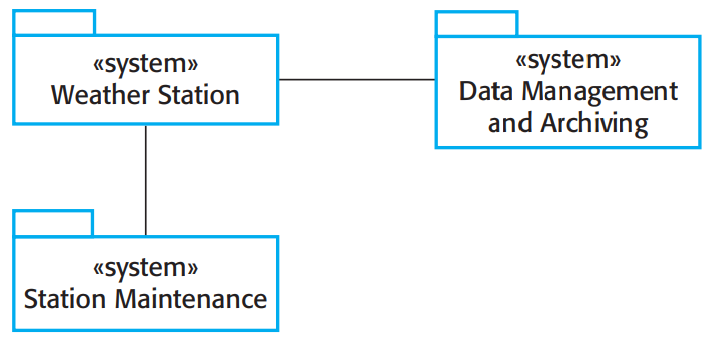
\includegraphics[width=0.45\linewidth]{images/weather-station-environment.PNG}
    \caption{L’ambiente della stazione meteorologica}
    \label{fig:weather-station-environment}
\end{figure}

I sistemi nella Figura \ref{fig:weather-station-environment} sono:
\begin{enumerate}
    \item \textit{Il sistema della stazione meteorologica:} Questo sistema è responsabile della raccolta dei dati meteorologici, dell'esecuzione di alcune elaborazioni iniziali dei dati e della trasmissione al sistema di gestione dei dati.
    \item \textit{Il sistema di gestione e archiviazione dei dati:} Questo sistema raccoglie i dati da tutte le stazioni meteorologiche selvagge, esegue l'elaborazione e l'analisi dei dati e archivia i dati in una forma recuperabile da altri sistemi.
    \item \textit{Il sistema di manutenzione delle stazioni:} Questo sistema può comunicare tramite satellite con tutte le stazioni meteorologiche selvagge per monitorare lo stato di salute di questi sistemi e fornire rapporti sui problemi.
\end{enumerate}
Il software della stazione non si occupa quindi solo della raccolta dei dati, ma deve anche:
\begin{enumerate}
    \item Monitorare gli strumenti, l'hardware di alimentazione e di comunicazione e segnalare i guasti al sistema di gestione.
    \item Gestire l'alimentazione del sistema, assicurandosi che le batterie vengano caricate ogni volta che le condizioni ambientali lo permettono, ma anche che i generatori vengano spenti in condizioni meteorologiche potenzialmente dannose, come venti forti.
    \item Consentire una riconfigurazione dinamica, in cui parti del software vengono sostituite con nuove versioni e gli strumenti di riserva vengono integrati nel sistema in caso di guasto del sistema.
\end{enumerate}

\subsection*{Ambiente di apprendimento digitale}
Un ambiente di apprendimento digitale è una piattaforma in cui può essere integrato un insieme di strumenti generici e specificamente progettati per l'apprendimento, oltre a una serie di applicazioni orientate ai bisogni degli studenti che utilizzano il sistema. Gli strumenti inclusi in ogni versione dell'ambiente vengono scelti dagli insegnanti e dagli studenti per soddisfare le loro specifiche esigenze. Questi strumenti possono includere applicazioni generali come fogli di calcolo, applicazioni di gestione dell'apprendimento come un ambiente virtuale di apprendimento (VLE) per gestire la consegna dei compiti e le valutazioni, giochi e simulazioni.

La Figura \ref{fig:architecture-digital-learning} è un modello architettonico ad alto livello di un ambiente di apprendimento digitale (iLearn). 

\begin{figure}[ht]
    \centering
    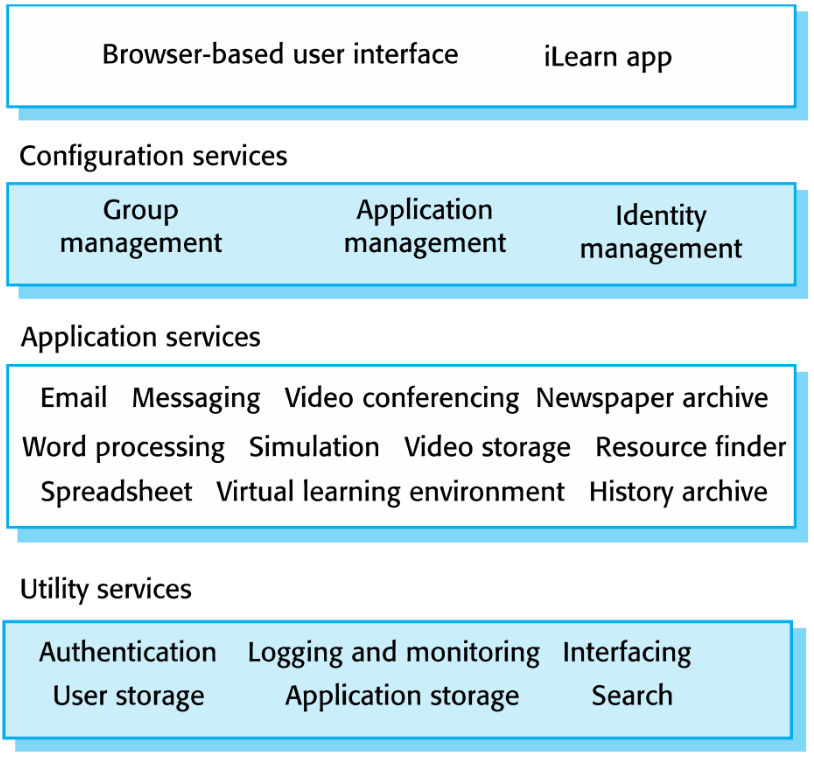
\includegraphics[width=0.5\linewidth]{images/architecture-digital-learning.PNG}
    \caption{L'architettura di un ambiente di apprendimento digitale}
    \label{fig:architecture-digital-learning}
\end{figure}

Il sistema è un sistema orientato ai servizi, in cui tutti i componenti del sistema sono considerati servizi sostituibili. Ci sono tre tipi di servizio nel sistema:
\begin{enumerate}
    \item \textit{Servizi di utilità:} Forniscono funzionalità di base indipendenti dalle applicazioni e possono essere utilizzati da altri servizi del sistema.
    \item \textit{Servizi applicativi:} Forniscono applicazioni specifiche come email, conferenze, condivisione di foto, ecc., e l'accesso a contenuti educativi specifici come film scientifici o risorse storiche.
    \item \textit{Servizi di configurazione:} Sono utilizzati per adattare l'ambiente con un set specifico di servizi applicativi e per definire come i servizi vengono condivisi tra studenti, insegnanti e genitori.
\end{enumerate}
L'ambiente è stato progettato in modo che i servizi possano essere sostituiti man mano che nuovi servizi diventano disponibili e per fornire versioni diverse del sistema adatte all'età degli utenti. Ciò significa che il sistema deve supportare due livelli di integrazione dei servizi:
\begin{enumerate}
    \item \textit{Servizi integrati:} Sono servizi che offrono un'API (interfaccia di programmazione delle applicazioni) e che possono essere accessibili da altri servizi tramite tale API. È quindi possibile una comunicazione diretta tra i servizi.
    \item \textit{Servizi indipendenti:} Sono servizi che vengono semplicemente accessibili tramite un'interfaccia del browser e che operano in modo indipendente dagli altri servizi. Le informazioni possono essere condivise con altri servizi solo tramite azioni esplicite dell'utente, come il copia e incolla; potrebbe essere richiesta una nuova autenticazione per ciascun servizio indipendente.
\end{enumerate}

\section{Punti chiave}
\begin{center}
\begin{minipage}{\textwidth}
\colorbox{lightgray}{
\parbox{\linewidth}{
\begin{itemize}
    \item L'ingegneria del software è una disciplina ingegneristica che si occupa di tutti gli aspetti della produzione del software. 
    \item Il software non è solo un programma o programmi, ma include anche tutta la documentazione elettronica necessaria per gli utenti del sistema, il personale di assicurazione della qualità e gli sviluppatori. Gli attributi essenziali di un prodotto software sono la manutenibilità, l'affidabilità e la sicurezza, l'efficienza e l'accettabilità. 
    \item Il processo di sviluppo del software include tutte le attività coinvolte nello sviluppo del software. Le attività ad alto livello di specifica, sviluppo, validazione ed evoluzione fanno parte di tutti i processi software. 
    \item Esistono molti tipi diversi di sistema, e ciascuno richiede strumenti e tecniche di ingegneria del software appropriati per il proprio sviluppo. Poche, se non nessuna, tecniche specifiche di progettazione e implementazione sono applicabili a tutti i tipi di sistema.
    \item Le idee fondamentali dell'ingegneria del software sono applicabili a tutti i tipi di sistema software. Questi fondamenti includono processi software gestiti, affidabilità e sicurezza del software, ingegneria dei requisiti e riuso del software. 
    \item Gli ingegneri del software hanno responsabilità nei confronti della professione ingegneristica e della società. Non dovrebbero occuparsi solo di questioni tecniche, ma dovrebbero essere consapevoli delle questioni etiche che influenzano il loro lavoro. 
    \item Le società professionali pubblicano codici di condotta che incorporano standard etici e professionali. Questi stabiliscono gli standard di comportamento attesi dai loro membri.
\end{itemize}
}}
\end{minipage}
\end{center}